\chapter{Related Work}
\label{chap:RelatedWork}

\section{The U-Net Architecture}

The article \emph{U-Net: Convolutional Networks for Biomedical Image Segmentation} (\cite{UNet}) introduces a fully-convolutional neural network, that is surprisingly good at performing image segmentation. The article uses this architecture for semantic segmentation and instance segmentation of various biomedical images.

\begin{figure}[ht]
    \centering
    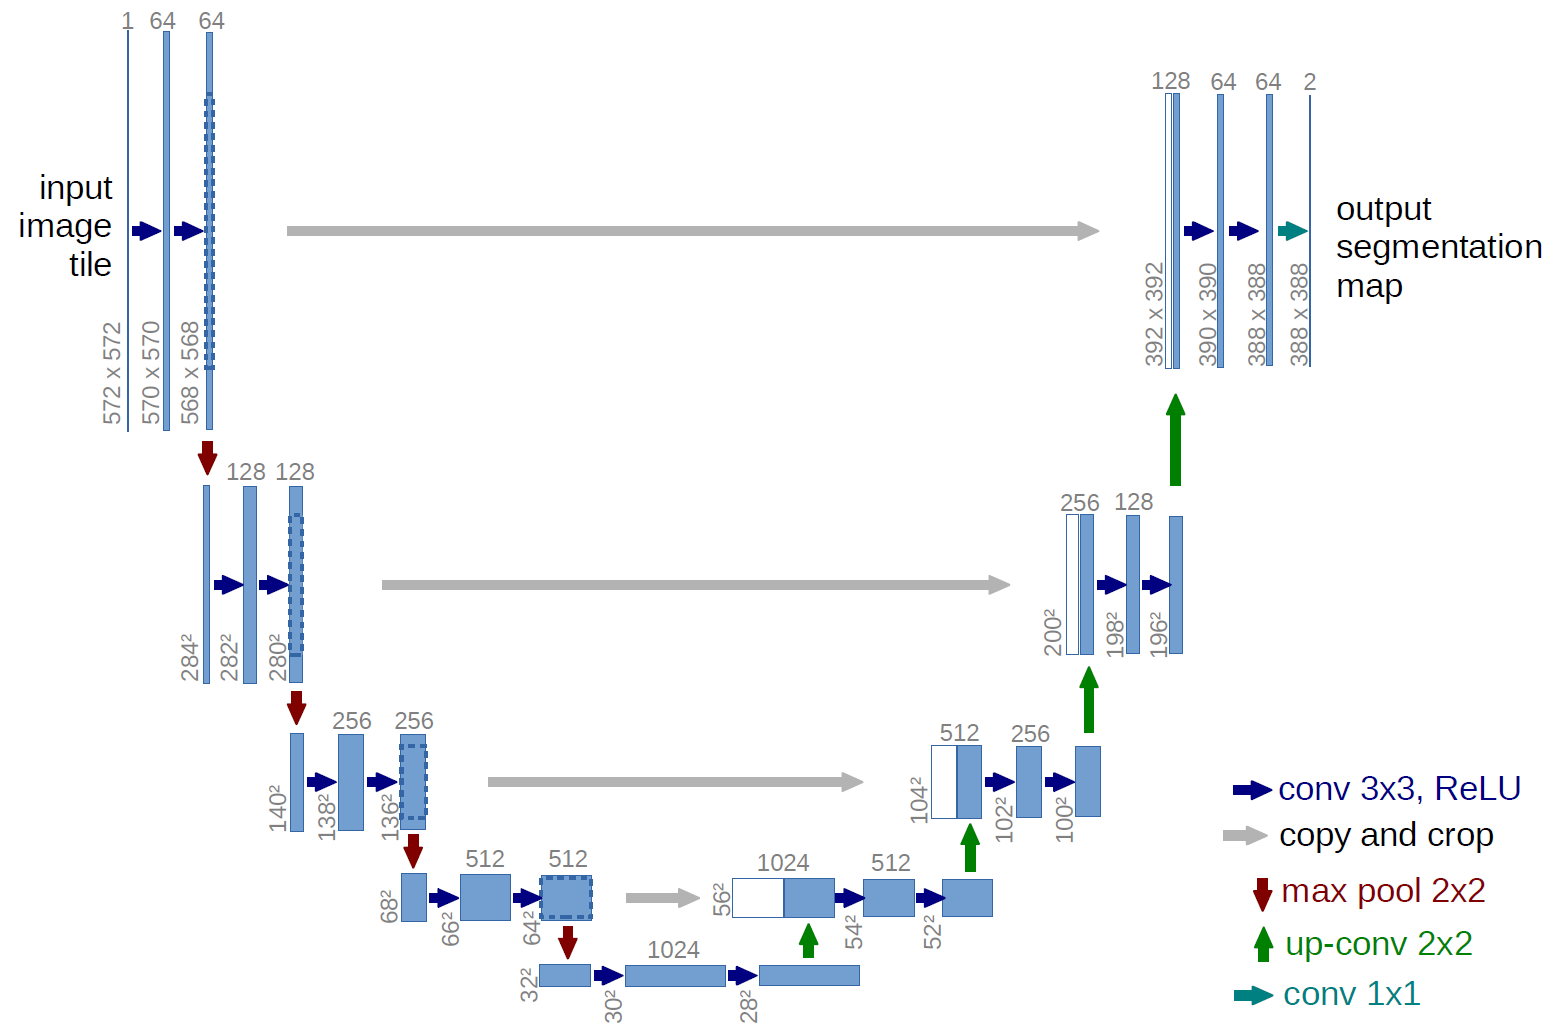
\includegraphics[width=145mm]{../img/u-net-architecture.png}
    \caption{The U-Net architecture with a contracting path and an expansive path. The image is taken from \cite{UNet}.}
    \label{fig:UNetArchitecture}
\end{figure}

The authors describe the left part of the network as the contracting path. It follows the typical structure of a convolutional network. The right part is called the expansive path. It is built as an inverse to the contractive part. The combination of contraction and expansion causes the network to first gather context information around each point of the image and then spread it back out to inform the segmentation process. The two halves are connected using skip-connections, so that the expansive path also has accurate local information available. Since the architecture resembles an autoencoder, we refer to the two halves of the network as an encoder and a decoder. One additional advantage of this architecture is its speed of both inference and training.


\section{Music Object Detection}

A variation of the U-Net architecture has been first utilized in the context of music recognition in the article \emph{On the Potential of Fully Convolutional Neural Networks for Musical Symbol Detection} (\cite{DorferEtAl}). Authors used it for notehead detection, as a continuation of their previous research into convolutional neural networks for music symbol detection. They managed to outperform other approaches with a much simpler system and faster inference time.

\begin{figure}[ht]
    \centering
    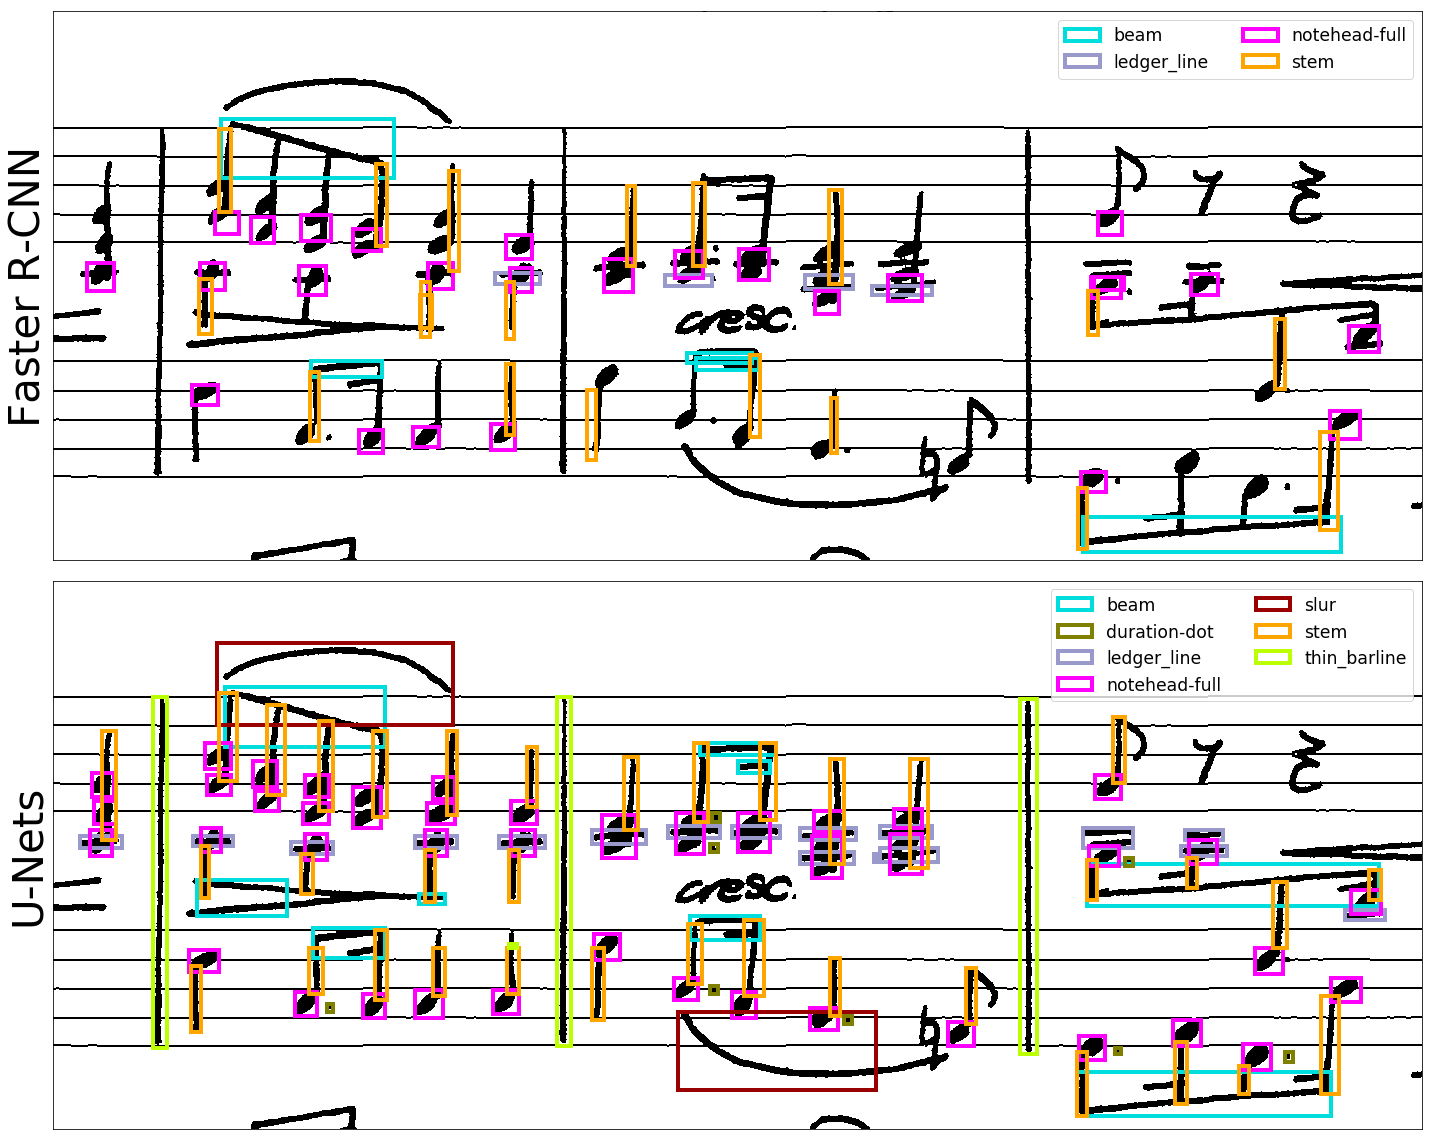
\includegraphics[width=145mm]{../img/muscima-detection-comparison.png}
    \caption{Comparison of the R-CNN and the U-Net architecture for object detection on the MUSCIMA++ dataset. The RetinaNet signle-shot detection is very poor, so the image is omitted to save space. The original image with additional images showing other datasets can be found in (\cite{PachaBaseline}).}
    \label{fig:MuscimaDetectionComparison}
\end{figure}

Both authors then refined the approach in the article \emph{Towards Full-Pipeline Handwritten OMR with Musical Symbol Detection by U-Nets} (\cite{HajicEtAl}). The architecture was extended to perform multi-class segmentation in one pass and domain-specific tricks have been added to increase performance on some symbols. A notation assembly system was designed using decision trees and a complete pipeline with MIDI output was constructed and evaluated.

In the same year, a comparison of object detection architectures for musical symbols was published: \emph{A Baseline for General Music Object Detection with Deep Learning} (\cite{PachaBaseline}). The authors trained three object detection architectures, namely Faster R-CNN, RetinaNet, and U-Net. Their evaluation was performed using three datasets with object detection ground truth, and varied appearance and content. These were the Capitan dataset (mensural notation), the DeepScores dataset (digitally printed modern notation), and the MUSCIMA++ dataset (handwritten modern notation). The article establishes baseline results in different areas of music recognition, but most importantly, identifies the U-Net architecture as the best known architecture for object detection.


\section{Generative Semi-supervised Learning}

The article \emph{Adversarial Autoencoders} (\cite{AdversarialAutoencoders}) proposes an autoencoder archtiecture, where the latent space distribution is shaped by an adversarial mechanism. A separate discriminator network is trained to distinguish between real embeddings from the dataset and fake embeddings drawn from the desired distribution. This process forces the encoder to produce embeddings that match the desired distribution (e.g.\@ gaussian). The resulting latent space is tightly filled with dataset embeddings and there are no holes present. This makes the decoder a very good generative model, as any random sample from the desired distribution will be correctly decoded into a realistic data point.

The article compares the latent space of an adversarial autoencoder (AAE) to a variational autoencoder (VAE) (\cite{VariationalAutoencoder}), and it is clearly visible how an AAE better matches a desired distribution. Most of these visualisations are performed on the MNIST dataset (\cite{Mnist}).

The article then describes modifications of the architecture, related to splitting the latent vector to a continuous and a categorical part and treating the categorical part as a class information. These modified archtiectures are then used to perfom many interesting tasks, such as semi-supervised classification, unsupervised clustering and styl-content disentangling.

The article is referenced here as a demonstration of the capabilities of generative semi-supervised models.

\begin{figure}[ht]
    \centering
    \begin{subfigure}{72.5mm}
        \raggedright
        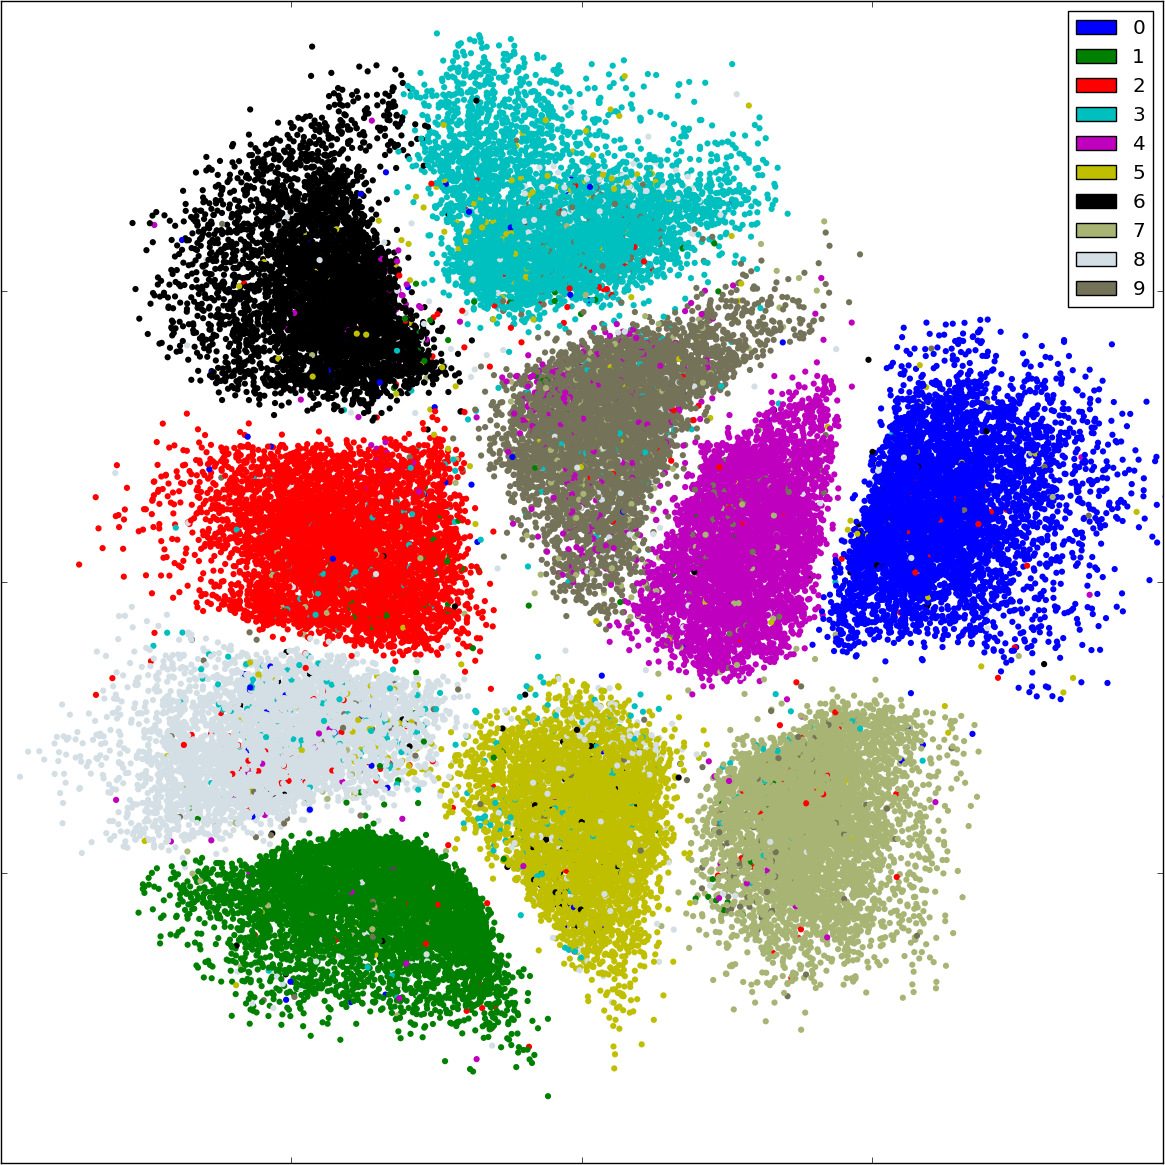
\includegraphics[width=70mm]{../img/aae-clustering-semi.png}
        \caption{semi-supervised, 1000 labels}
    \end{subfigure}%
    \begin{subfigure}{72.5mm}
        \raggedleft
        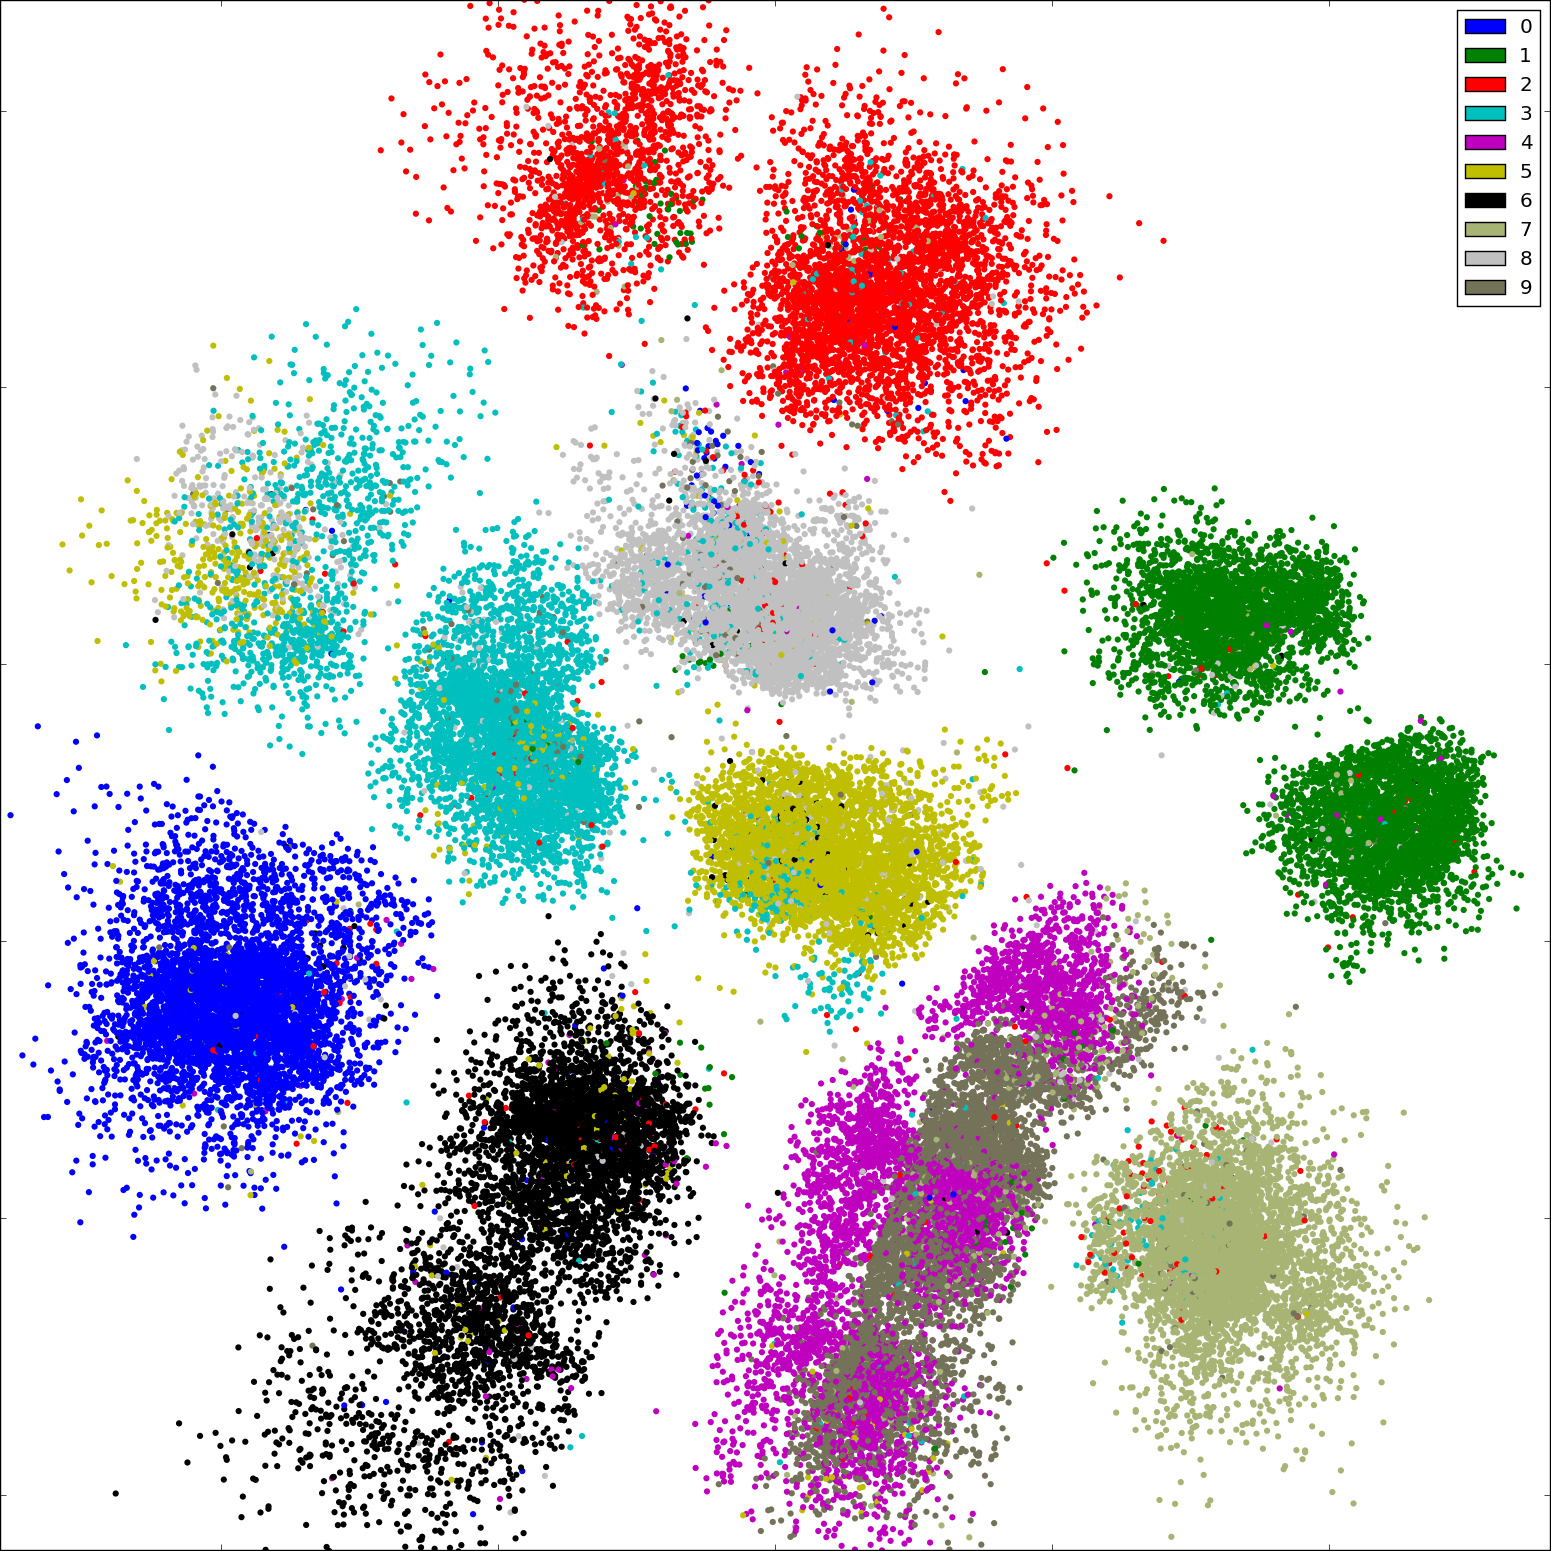
\includegraphics[width=70mm]{../img/aae-clustering-unsup.png}
        \caption{unsupervised}
    \end{subfigure}
    \caption{Semi-supervised and unsupervised dimensionality reduction results for an adversarial autoencoder on the MNIST dataset. Images taken from \cite{AdversarialAutoencoders}.}
    \label{fig:test}
\end{figure}

